\chapter{绪论}
\section{研究背景}
天下武功,无坚不破,唯快不破。灵犀一指属于快而非坚之武学。


\section{本论文的工作}
本论文的研究对象为灵犀一指,着重研究其中的内功心法。
%正文内容,引用参考文献
详见文献\cite{Peebles2001-100-100}\parencite{Babu2014--}
参考文献\cite[见][49页]{于潇2012-1518-1523}\parencite[见][49页]{Babu2014--}
硕士论文\cite{zhouGPS2015},博士论文\cite{余勇1998--}
大小写\cite{liu_statistical_2017}

\nomenclature{PF}{powerful fingers}
如图\ref{lxfbook}所示。

\begin{figure}
    \centering
    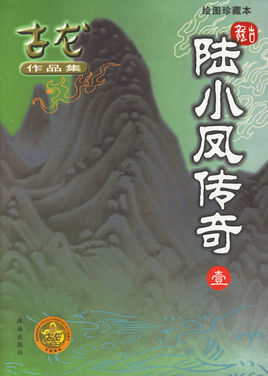
\includegraphics[width=.6\textwidth]{lxfbook.jpg}
    \caption{陆小凤传奇\label{lxfbook}}
\end{figure}
\nomenclature{KF}{kung fu}